\section{Affine and Projective Spaces}

\subsection{Affine Spaces}

  Modeling the space of points as a vector space can be unsatisfactory for a number of reasons. 
  \begin{enumerate}
    \item The origin $0$ plays a special role, when it doesn't necessarily need to have one. 
    \item Certain notions, such as parallelism, are handled in an awkward manner. 
    \item The geometries of vector and affine spaces are intrinsically. That is, 
      \begin{equation}
        \GL(V) \subset \GA(V)
      \end{equation}
  \end{enumerate}

  In the ordinary Euclidean geometry, one can define the operation of the addition of a point and a vector. That is, the "sum" of a point $p$ and a vector $x$ is the endpoint of a vector that starts at $p$ and equals $x$. We formalize it in the following definition. 

  \begin{definition}
    Let $V$ be a vector space over field $\mathbb{F}$. The \textbf{affine space associated to $V$} is a set $S$ with an operation of addition $+: S \times V \longrightarrow S$ satisfying 
    \begin{enumerate}
      \item $p + (x + y) = (p + x) + y$ for $p \in S, x, y \in V$
      \item $p + 0 = p$ where $p \in S$, $0$ is the zero vector 
      \item For any $p, q \in S$, there exists a unique vector $x$ such that $p + x = q$
    \end{enumerate}
    Elements of the set $S$ are called \textbf{points}. The vector in condition 3 is called the \textbf{vector connecting points $p$ and $q$}, denoted $\overline{pq}$. The dimension of an affine space is defined as the dimension of the corresponding vector space. 
  \end{definition}

  The first condition implies that
  \begin{equation}
    \overline{pq} + \overline{qr} = \overline{pr} \text{ for all } p, q, r \in S
  \end{equation}
  Every vector space $V$ can be regarded as an affine one if we view vectors both as points and as points and define the operation of addition of a vector to a point as addition of vectors. Under this interpretation, the vector $\overline{pq}$ is the difference between the vectors $p$ and $q$. 

  \begin{definition}
    Conversely, if we fix a point $o$ (the origin) in an affine space $S$, we can identify a point $p$ with its \textbf{position vector} $\overline{op}$. Then, addition of a vector to a point just becomes the addition a vectors. This identification of points with vectors is called the \textbf{vectorization} of an affine space. 
  \end{definition}

  \begin{definition}
    A point $o$ (the origin) together with a basis $\{e_1, ..., e_n\}$ of the space $V$ is called a \textbf{frame} of the affine space $S$. Each frame is related to an \textbf{affine system of coordinates} in the space $S$. That is, a point $p$ would get the coordinates equal to those of the vector $\overline{op}$ in the basis $\{e_1, ..., e_n\}$. It is easy to see that 
    \begin{enumerate}
      \item Coordinates of the point $p+x$ are equal to the sums of respective coordinates of the point $p$ and the vector $x$. 
      \item Coordinates of the vector $\overline{pq}$ are equal to the differences of respective coordinates of the points $q$ and $p$. 
    \end{enumerate}
  \end{definition}

  Linear combinations of points are not defined in the affine space since the values of linear combinations are actually dependent on the choice of the origin. However, an analogous structure can be. 

  \begin{definition}
    The \textbf{barycentric linear combination} of points $p_1, ..., p_k \in S$ is a linear combination of the form
    \begin{equation}
      p = \sum_i \lambda_i p_i, \text{ where } \sum_i \lambda_i = 1
    \end{equation}
    This linear combination is equal to the point $p$ such that
    \begin{equation}
      \overline{op} = \sum_i \lambda_i \overline{op_i}
    \end{equation}
    where $o \in S$ is any origin point.
  \end{definition}

  \begin{definition}
    In particular, the specific barycentric combination of points where $\lambda_1 = ... = \lambda_k = \frac{1}{k}$ is called the \textbf{center of mass} of the collection of points $p_i$. 
  \end{definition}

  \begin{definition}
    Let $p_0, p_1, ..., p_n$ be points of an $n$-dimensional affine space $S$ such that the vectors $\overline{p_0 p_1}, ..., \overline{p_0 p_n}$ are linearly independent (that is, forms a basis). Then, every point $p \in S$ can be uniquely presented as 
    \begin{equation}
      p = \sum_{i=0}^n x_i p_i, \text{ where } \sum_{i=0}^n x_i = 1
    \end{equation}
    This equality can be rewritten
    \begin{equation}
      \overline{p_0 p} = \sum_{i=1}^n x_i \overline{p_0 p_i}
    \end{equation}
    implying that we can take the coordinates of the vector $\overline{p_0 p}$ in the basis $\{ \overline{p_0 p_1}, ..., \overline{p_0 p_n}\}$ as $x_1, ..., x_n$. Then, $x_0$ is determined as 
    \begin{equation}
      x_0 = 1 - \sum_{i=1}^n x_i
    \end{equation}
    The numbers $x_0, x_1, ..., x_n$ are called the \textbf{barycentric coordinates} of the point $p$ with respect to $p_0, p_1, ..., p_n$. 
  \end{definition}

  \begin{definition}
    A \textbf{plane} in an affine space $S$ is a subset of the form 
    \begin{equation}
      p = p_0 + U
    \end{equation}
    where $p_0$ is a point and $U$ is a subspace of the space $V$. Note that we can choose any point $p_0$ in the plane in this representation. $U$ is called the \textbf{direction subspace} for $P$. 
  \end{definition}

  \begin{lemma}
    If the intersection of two planes in an affine space is nonempty, then the intersection is also a plane. 
  \end{lemma}

  \begin{theorem}
    Given any $k+1$ points of an affine space, there is a plane of dimension $\leq k$ passing through these points. If these points are not contained in a plane of dimension $< k$, then there exists a unique $k$-dimensional plane passing through them. 
  \end{theorem}

  \begin{definition}
    Points $p_0, p_1, ..., p_k \in S$ are \textbf{affinely dependent} if they lie in a plane of dimension $<k$, and \textbf{affinely independent} otherwise. It is clear that the points $p_0,..., p_k$ are affinely independent if and only if the vectors $\overline{p_0p_1}, ..., \overline{p_0 p_k}$ are linearly independent. 
  \end{definition}

  \begin{theorem}
    Points $p_0, ..., p_k \in S$ are affinely independent if and only if the rank of the matrix of their barycentric coordinates (with respect to some predetermined affinely independent points) equals $k+1$. 
  \end{theorem}

  It is easy to see that the previous theorem is true, since the determinant represents the hypervolume of the parallelopiped spanned by the vectors $\overline{p_0p_1}, ..., \overline{p_0 p_k}$, which must be nonzero if they are indeed affinely independent. 

  \begin{corollary}[Menelaus' Theorem]
    Let points $x, y, z$ line on the sides $bc, ca, ab$ of the triangle $abc$ or their continuations. 
    \[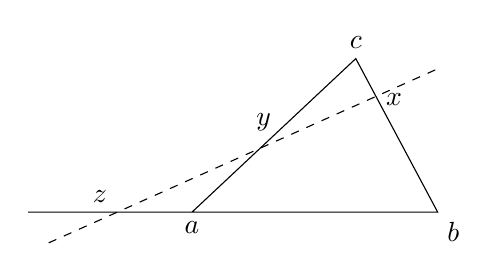
\begin{tikzpicture}[scale=1.3]
      \draw (-1,0)--(3,0)--(2.2, 1.5)--(0.6,0);
      \node[below] at (0.6, 0) {$a$};
      \node[below right] at (3,0) {$b$};
      \node[above] at (2.2, 1.5) {$c$};
      \draw[dashed] (-0.8,-0.3)--(3,1.4);
      \node[above] at (-0.3, 0) {$z$};
      \node[above] at (1.3, 0.7) {$y$};
      \node[right] at (2.4, 1.1) {$x$};
    \end{tikzpicture}\]
    Suppose that they divide these sides in the ratio 
    \[\lambda: 1, \mu: 1, \nu: 1\]
    respectively. Then, the points $x, y, z$ lie on the same line if and only if 
    \[\lambda \mu \nu = -1\]
  \end{corollary}
  \begin{proof}
  By the previous theorem, the points $x, y, z$ are linearly dependent (i.e. lies on a line) if and only if the matrix of barycentric coordinates of $x, y, z$ with respect to $a, b, c$, which is
  \begin{equation}
    \begin{pmatrix}
    0 & \frac{1}{\lambda + 1} & \frac{\lambda}{\lambda + 1} \\
    \frac{\mu}{\mu + 1} & 0 & \frac{1}{\mu + 1} \\
    \frac{1}{\nu + 1} & \frac{\nu}{\nu+1} & 0
    \end{pmatrix}
  \end{equation}
  has nonzero determinant. The determinant of the above matrix is $0$ if and only if $\lambda \mu \nu = -1$. 
  \end{proof}

  \begin{corollary}[Ceva's Theorem]
    In the triangle above, the lines $ax, by, cz$ intersect at one point if and only if 
    \begin{equation}
      \lambda \mu \nu = 1
    \end{equation}
  \end{corollary}
  \begin{proof}
    The proof can be done using barycentric coordinates. 
  \end{proof}

  \begin{theorem}
    A nonempty subset $P \subset S$ is a plane if and only if for any two distinct points $a, b \in P$, the line through $a$ and $b$ also lies in $P$. 
  \end{theorem}

  \begin{theorem}
    Given an inhomogeneous system of linear equations of form 
    \begin{equation}
      A x = b
    \end{equation}
    the set of solutions is an affine plane of dimension $n-r$, where $n$ is the number of variables and $r$ is the rank of the matrix $A$. More precisely, given that the plane is in the form $P = p_0 + U$, $p_0$ is one solution and $U$ is the set of vectors that satisfy the homogeneous system
    \begin{equation}
      Ax = 0
    \end{equation}
  \end{theorem}

  Let us observe the relative position of two planes. 

  \begin{theorem}
    Given two planes 
    \begin{align*}
      P_1 = p_1 + U_1, & P_2 = p_2 + U_2
    \end{align*}
    $P_1$ and $P_2$ intersect if and only if 
    \begin{equation}
      \overline{p_1 p_2} \subset U_1 + U_2
    \end{equation}
    where $U_1 + U_2$ is the set of all vectors of form $u_1 + u_2$, where $u_1 \in U_1, u_2 \in U_2$. 
  \end{theorem}

  Now, consider the class of functions on an affine space corresponding to the class of linear functions on a vector space. 

  \begin{definition}
    An \textbf{affine-linear} function on an affine space $S$ is a function $f: S \longrightarrow \mathbb{F}$ such that
    \begin{equation}
      f(p + x) = f(p) + \alpha (x), \;\; p \in S , x \in V
    \end{equation}
    where $\alpha$, called the \textbf{differential}, is a linear function on the vector space $V$. Let $o \in S$ be a fixed origin. By setting $p = o$, we can express an affine linear function in vectorized form as 
    \begin{equation}
      f(x) = \alpha (x) + b, \;\; b \in \mathbb{F}
    \end{equation}
    where $b = f(o)$. This implies the following coordinate form of $f$. 
    \begin{equation}
      f(x) = b + \sum_i a_i x_i
    \end{equation}
  \end{definition}

  A particular case of affine-linear functions are constant functions, where the defining characteristic is the zero differential. 

  \begin{theorem}
    Given that $\dim{S} = n$, affine-linear functions on $S$ form a $(n+1)$-dimensional subspace on the space of all linear functions on $S$. 
  \end{theorem}

  \begin{theorem}
    Barycentric coordinates are affine-linear functions. 
  \end{theorem}

  \begin{theorem}
    Let $f$ be an affine-linear function. Then
    \begin{equation}
      f \bigg( \sum_i \lambda_i p_i \bigg) = \sum_i \lambda_i f(p_i)
    \end{equation}
    for any barycentric linear combination $\sum_i \lambda_i p_i$ of points $p_1, ..., p_k$. 
  \end{theorem}

  \begin{definition}
    An affine space associated with a Euclidean vector space is called a \textbf{Euclidean affine space}. The \textbf{distance $\rho$} between two points in a Euclidean space is defined as
    \begin{equation}
      \rho(p, q) = ||\overline{pq}||
    \end{equation}
    This definition of $\rho$ satisfies the axioms of a metric space. 
  \end{definition}

\subsection{Convex Sets}

  Let $S$ be an affine space over the field of real numbers and $V$, the associated vector space. 

  \begin{definition}
    The \textbf{(closed) interval} connecting points $p, q \in S$ is the set
    \begin{equation}
      pq = \{\lambda p + (1-\lambda) q \;|\; 0 \leq \lambda \leq 1\}
    \end{equation}
    Geometrically, we can think of this as the straight line segment connecting point $p$ with point $q$. 
  \end{definition}

  \begin{definition}
    A set $M \subset S$ is \textbf{convex} if for any two points $p, q \in S$, it contains the whole interval $p, q$. 
  \end{definition}

  Clearly, the intersection of convex sets is convex. However, the union of them is not. 

  \begin{definition}
    A \textbf{convex linear combination} of points in $S$ is their barycentric linear combination with nonnegative coefficients. 
  \end{definition}

  It is clear to visualize the following theorem. 

  \begin{theorem}
    For any points $p_0, ..., p_k$ in a convex set $M \subset S$, the set $M$ also contains every convex linear combination 
    \begin{equation}
      p = \sum_i \lambda_i p_i
    \end{equation}
    Furthermore, for any set $M \subset S$, the set $\conv{M}$ of all convex linear combinations of points in $M$ is convex. 
  \end{theorem}

  \begin{definition}
    Given $M \subset S$, the set $\conv M$ is the smallest convex set containing $M$. It is called the \textbf{convex hull} of $M$. 
  \end{definition}

  \begin{definition}
    The convex hull of a system of affinely independent points $p_0, p_1, ..., p_n$ in an $n$-dimensional affine space is called the \textbf{$n$-dimensional simplex} with vertices $p_0, ..., p_n$. 
  \end{definition}

  It is clear that the interior points of a simplex is precisely the set of all points whose barycentric coordinates with respect to the vertices are all positive. 

  \begin{example}
    Here are common examples of simplices.
    \begin{enumerate}
      \item A $0$-dimensional simplex is a point. 
      \item A $1$-dimensional simplex is a closed line interval. 
      \item A $2$-dimensional simplex is a triangle. 
      \item A $3$-dimensional simplex is a tetrahedron. 
    \end{enumerate}
  \end{example}

  \begin{theorem}
    A convex set $M$ has interior points if and only if $\aff M = S$. 
  \end{theorem}

  \begin{definition}
    A convex set that has interior points is called a \textbf{convex body}. Clearly, every convex body in $n$-dimensional affine space $S$ is $n$-dimensional. 
  \end{definition}

  The set of interior points of a convex body $M$, denoted $M^\circ$, is an open convex body. 

  \begin{definition}
    For any nonconstant affine-linear function $f$ on the set $S$, let
    \begin{align*}
      H_f \equiv \{p \in S \;|\; f(p) = 0\} \\
      H^+_f \equiv \{p \in S \;|\; f(p) \geq 0\} \\
      H^-_f \equiv \{p \in S \;|\; f(p) \leq 0\}
    \end{align*}
    The set $H_f$ is a hyperplane, and $H^+_f, H^-_f$ are called \textbf{closed half spaces}. 
  \end{definition}

  \begin{definition}
    A hyperplane $H_f$ is a \textbf{supporting hyperplane} of a closed convex body $M$ if $M \subset H^+_f$ and $H_f$ contains at least one (boundary) point of $M$. The half space $H^+_f$ is then called the \textbf{supporting half-space} of $M$. 
  \end{definition}

  \begin{theorem}
    A hyperplane $H$ that passes through a boundary point of a closed convex body $M$, is supporting if and only if $H \cap M^\circ = \emptyset$. 
  \end{theorem}

  A key theorem of convex sets is the following separation theorem. 

  \begin{theorem}[Separation Theorem]
    For every boundary point of a closed convex body, there exists a supporting hyperplane passing through this point. 
  \end{theorem}

  This theorem leads to the following one. 

  \begin{theorem}
    Every closed convex set $M$ is an intersection of (perhaps infinitely many) half-spaces. 
  \end{theorem}

  \begin{definition}
    A \textbf{polyhedron} is the intersection of a finite number of half-spaces. A convex polyhedron which is also a body is called a \textbf{convex solid}. 
  \end{definition}

  \begin{example}
    A simplex with vertices $p_0, p_1, ..., p_n$ is a convex polyhedron since it is determined by linear inequalities $x_i \geq 0$ for $i = 0, 1, ..., n$, where $x_0, x_1, ..., x_n$ are barycentric coordiantes with respect to $p_0, p_1,..., p_n$. 
  \end{example}

  \begin{example}
    A convex polyhedron determined by linear inequalities $0 \leq x_i \leq 1$ for $i = 1, ..., n$, where $x_1,..., x_n$ are affine coordinates with respect ot some frame, is called an $n$-dimensional parallelopiped. 
  \end{example}

  \begin{definition}
    A point $p$ of a convex set $M$ is \textbf{extreme} if it is not an interior point of any interval in $M$. 
  \end{definition}

  \begin{theorem}
    A bounded closed convex set $M$ is the convex hull of the set $E(M)$ of its extreme points. 
  \end{theorem}

  We can create a stronger statement with the following theorem. 

  \begin{theorem}[Minkowski-Weyl Theorem]
    The following properties of a bounded set $M \subset S$ is equivalent.
    \begin{enumerate}
      \item $M$ is a convex polyhedron. 
      \item $M$ is a convex hull of a finite number of points. 
    \end{enumerate}
  \end{theorem}

  \begin{definition}
    A \textbf{face} of a convex polyhedron $M$ is a nonempty intersection of $M$ with some of its supporting hyperplanes. Given that $\dim \aff M = n$, 
    \begin{enumerate}
      \item A $0$-dimensional face is called a \textbf{vertex}. 
      \item A $1$-dimensional face an \textbf{edge}. 
      \item ...
      \item An $(n-1)$-dimensional face a \textbf{hyperface}. 
    \end{enumerate}
  \end{definition}

  Therefore, if a convex polyhedron is determined by a system of linear inequalities, we can obtain its faces by replacing some of these inequalities with equalities (in such a way that we do not get the empty set). 

  The following theorem demonstrates that in order to find its faces, it suffices to consider only the hyperplanes $H_{f_1}, ..., H_{f_m}$. 

  \begin{theorem}
    Every face $\Gamma$ of the polyhedron $M$ is of the form
    \begin{equation}
      \Gamma = M \cap \bigg( \bigcap_{j \in J} H_{f_j} \bigg)
    \end{equation}
    where $J = \{1, 2, ..., m\}$
  \end{theorem}

  \begin{theorem}
    The extreme points of a convex polyhedron $M$ are exactly its vertices. 
  \end{theorem}

  The following theorem is used often in linear programming and in optimization. 

  \begin{theorem}
    The maximum of an affine-linear function on a bounded convex polyhedron $M$ is attained at a vertex. 
  \end{theorem}

\subsection{Affine Transformations and Motions}

  Let $S$ and $S^\prime$ be affine spaces associated with vector spaces $V$ and $V^\prime$, respectively, over the same field $\mathbb{F}$. 

  \begin{definition}
    An \textbf{affine map} from the space $S$ to the space $S^\prime$ is a map $f: S \longrightarrow S^\prime$ such that
    \begin{equation}
      f(p+x) = f(p) + \varphi(x), \;\; p \in S, x \in V
    \end{equation}
    for some linear map $\varphi: V \longrightarrow V^\prime$. It follows that
    \begin{equation}
      \varphi(\overline{pq}) = \overline{f(p) f(q)}, \;\; p, q \in S
    \end{equation}
    Thus, $f$ determines the linear map $\varphi$ uniquely. Similarly, $\varphi$ is called the \textbf{differential} of $f$, denoted $df$. 
  \end{definition}

  \begin{theorem}
    Let $f: S \longrightarrow S^\prime$ and $g: S^\prime \longrightarrow S^{\prime \prime}$ be two affine maps. Then the map
    \begin{equation}
      g \circ f : S \longrightarrow S^{\prime\prime}
    \end{equation}
    is also affine. Also
    \begin{equation}
      d(g \circ f) = dg \cdot df
    \end{equation}
    where $dg$ and $df$ are the differentials of $g$ and $f$, respectively. 
  \end{theorem}

  For $\mathbb{F} = \mathbb{R}$, the differential of an affine map is a particular case of a differential of a smooth map in analysis. That is, the differential is the linear approximation of the function $f$. 

  \begin{theorem}
    An affine map is bijective if and only if its differential is bijective. 
  \end{theorem}

  \begin{definition}
    Similar to linear transformations between vector spaces, bijective affine transformations are called \textbf{isomorphisms} of affine spaces. Affine spaces are \textbf{isomorphic} if there exists an isomorphism between them. 
  \end{definition}

  \begin{corollary}
    Finite-dimensional affine spaces over the same field are isomorphic if and only if they have the same dimension. 
  \end{corollary}

  \begin{definition}
    An affine map from an affine space $S$ to itself is called an \textbf{affine transformation}. Bijective affine transformations form a group called the \textbf{affine group of $S$}, denoted $\GA(S)$. 
  \end{definition}

  It follows that given affine space $S$ with associated vector space $V$, the projection map
  \begin{equation}
    d: \GA(S) \longrightarrow \GL(V)
  \end{equation}
  is a group homomorphism. It's kernel is the group of parallel translations, called Tran$(S)$. 
  \begin{equation}
    t_a : p \mapsto p + a, \;\; a \in V
  \end{equation}

  \begin{theorem}
    For any $f \in \GA(S)$ and $a \in V$, 
    \begin{equation}
      f t_a f^{-1} = t_{df(a)}
    \end{equation}
  \end{theorem}

  \begin{definition}
    A \textbf{homothety} with the center $o$ and coefficient $\lambda$ is an affine transformation defined as
    \begin{equation}
      f( o + x ) \equiv o + \lambda x
    \end{equation}
    In its vectorized form, it is expressed
    \begin{equation}
      f(x) = \lambda x + b, \;\; b \in V
    \end{equation}
    A homothety with coefficient $-1$ is called a \textbf{central symmetry}. 
  \end{definition}

  The group of affine transformations determines the \textbf{affine geometry} of the space. The following theorem shows that all simplices are equal in affine geometry. 

  \begin{theorem}
    Let $\{p_0, ..., p_n\}$ and $\{q_0, ..., q_n\}$ be two systems of affinely independent points in an $n$-dimensional affine space $S$. Then there exists a unique affine transformation $f$ that maps $p_i$ to $q_i$ for $i = 0, 1, ..., n$. 
  \end{theorem}
  \begin{proof}
    It is easy to see once we realize that there exists a unique linear map $\varphi$ of the space $V$ that maps the basis $\{\overline{p_0 p_1}, ..., \overline{p_0 p_n}\}$ to the basis $\{\overline{q_0 q_1}, ..., \overline{q_0 q_n}\}$. If we vectorize $S$ by taking $p_0$ as the origin, the affine transformation in question has the form 
    \begin{equation}
      f(x) = \varphi(x) + \overline{p_0 q_0}
    \end{equation}
  \end{proof}

  \begin{corollary}
    In real affine geometry all parallelopipeds are equal. 
  \end{corollary}

  \begin{definition}
    A \textbf{motion} of the space $S$ is an affine transformation of $S$ whose differential is an orthogonal operator (i.e. an origin preserving isometry). Every motion is bijective. 
  \end{definition}

  Motions of a Euclidean space $S$ form a group denoted Isom$\,S$. A motion is called \textbf{proper (orientation preserving)} if its differential belongs to SO$(V)$ and improper otherwise. 

  \begin{lemma}
    The group Isom$\,S$ is generated by reflections through hyperplanes. 
  \end{lemma}

  \begin{definition}
    Let $M$ be a solid convex polyhedron in an $n$-dimensional Euclidean space. A \textbf{flag of $M$} is a collection of its faces $\{F_0, F_1, ..., F_{n-1}\}$ where $\dim{F_k} = k$ and $F_0 \subset F_1 \subset ... \subset F_{n-1}$. 
  \end{definition}

  \begin{definition}
    A convex polyhedron $M$ is \textbf{regular} if for any two of its flags, there exists a motion $f \in$ Sym$\,M$ mapping the first to the second, where 
    \begin{equation}
      \text{Sym}\,M \equiv \{f \in \text{Isom}\,S \;|\; f(M) = M \}
    \end{equation}
  \end{definition}

  Two dimensional regular polyhedra are the ordinary \textbf{regular polygons}. Their symmetry groups are known as the dihedral groups.

  Three dimensional regular polyhedra are \textbf{Platonic solids}, which are the regular tetrahedron, cube, octahedron, dodecahedron, and icosahedron. 

  \begin{definition}
    A real vector space $V$ with a fixed symmetric bilinear function $\alpha$ of signature $(k, l)$, where $k, l > 0$ and $\dim{V} = k+l$, is called the \textbf{pseudo-Euclidean vector space} of signature $(k, l)$. The group of $\alpha$-preserving linear transformations of $V$ is called the \textbf{pseudo-orthogonal group} and is denoted O$(V, \alpha)$. In an orthonormal basis, the corresponding matrix group is denoted $O{k,l}$. 
  \end{definition}

\subsection{Quadrics}

  Planes are the simplest objects of affine and Euclidean geometry, which are determined by systems of linear equations. The second simplest are quadratic functions. These types of objects are studied futher in algebraic geometry. 

  \begin{definition}
    An \textbf{affine-quadratic function} on an affine space $S$ is a function $Q: S \longrightarrow \mathbb{F}$ such that its vectorized form is
    \begin{equation}
      Q(x) = q(x) + l(x) + c
    \end{equation}
    for a quadratic function $q$, linear function $l$, and constant $c$. 
  \end{definition}

\subsection{Projective Spaces}

  \begin{definition}
    An $n$-dimensional \textbf{projective space $PV$} over a field $\mathbb{F}$ is the set of one-dimensional subspaces of an $(n+1)$-dimensional vector space $V$ over $\mathbb{F}$. For every $(k+1)$-dimensional subspace $U \subset V$, the subset $PU \subset PV$ is called a $k$-dimensional \textbf{plane} of the space $PV$. 
    \begin{enumerate}
      \item $0$-dimensional planes are the points of $PV$. 
      \item $1$-dimensional planes are called \textbf{lines}
      \item ...
      \item $(n-1)$-dimensional planes are called \textbf{hyperplanes}
    \end{enumerate}
  \end{definition}

  \begin{definition}
    $\mathbb{RP}^1$ is called the real projective line, which is topologically equivalent to a circle. 
  \end{definition}

  \begin{example}
    The real projective space of $\mathbb{R}^2$ is the set of all lines that pass through the origin. It is denoted $\mathbb{R P}^2$ and called the \textbf{real projective plane}. 
  \end{example}

  \begin{example}
    $\mathbb{RP}^3$ is diffeomorphic to SO$(3)$. 
  \end{example}

  \begin{example}
    The space $\mathbb{RP}^n$ is formed by taking the quotient of $\mathbb{R}^{n+1} \setminus \{0\}$ under the equivalence relation 
    \begin{equation}
      x \sim \lambda x \text{ for all real numbers } \lambda \neq 0
    \end{equation}
    The set of these equivalence classes is isomorphic to $\mathbb{RP}^n$. 
  \end{example}

